\documentclass{standalone}
\usepackage{tikz}
\usetikzlibrary{calc}
\begin{document}

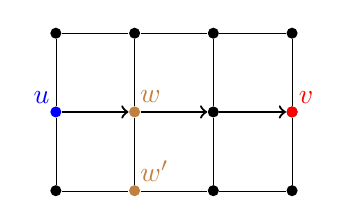
\begin{tikzpicture}[
  every node/.style={circle, fill=black, inner sep=1pt, minimum size=4pt}
]

  \node (a) at (0,6) {};
  \node (b) at (1,6){};
  \node (c) at (2,6){};
  \node (d) at (3,6){};
  \node[label={[blue]above left:$u$}] (e) at (0,5) [circle, color=blue] {};
  \node[label={[brown]above right:$w$}] (f) at (1,5) [circle, color=brown] {};
  \node (g) at (2,5){};
  \node (h) at (3,5){};
  \node[label={[red]above right:$v$}] (h) at (3,5) [circle, color=red] {};
  \node (i) at (0,4){};
  \node[label={[brown]above right:$w'$}] (j) at (1,4) [circle, color=brown] {};
  \node (k) at (2,4){};
  \node (l) at (3,4){};

  \draw (a) edge[-, ultra thin] (b);
  \draw (a) edge[-, ultra thin] (e);
  \draw (b) edge[-, ultra thin] (c);
  \draw (b) edge[-, ultra thin] (f);
  \draw (c) edge[-, ultra thin] (d);
  \draw (c) edge[-, ultra thin] (g);
  \draw (d) edge[-, ultra thin] (h);
  \draw (e) edge[-, ultra thin] (i);
  \draw (i) edge[-, ultra thin] (j);
  \draw (f) edge[-, ultra thin] (j);
  \draw (j) edge[-, ultra thin] (k);
  \draw (g) edge[-, ultra thin] (k);
  \draw (k) edge[-, ultra thin] (l);
  \draw (h) edge[-, ultra thin] (l);
  \draw (e) edge[->, thick] (f);
  \draw (f) edge[->, thick] (g);
  \draw (g) edge[->, thick] (h);

\end{tikzpicture}

\end{document}
